% !Mode:: "TeX:UTF-8"

\chapter[k-means并行化]{k-means并行化}
\section{k-means算法介绍}
    k-means聚类算法的核心是将分散的数据点分类或者聚集成k个组中,其中k是组别的数目。聚类算法的中心思想是
初始化每个组的中心点,并依次计算剩余数据点与每个组中心点的距离(其中距离可以使用Euclidean距离来衡量)
。每个数据点被分配到距离最近的组中,然后更新此分组的中心点,直到整个数据集中分组的中心点不再变化为止.
选择每个组的初始中心点有三种方法:动态选择,随机选择,根据数据集中最大值和最小值。

   kmeans算法核心,如图~\ref{fig:kmeans1}所示,其中黑色点表示待聚类的数据点,红色表示k-means算法实现的分组
情况,蓝色表示每个分组内的中心点

    \begin{figure}[htbp]
    \centering
    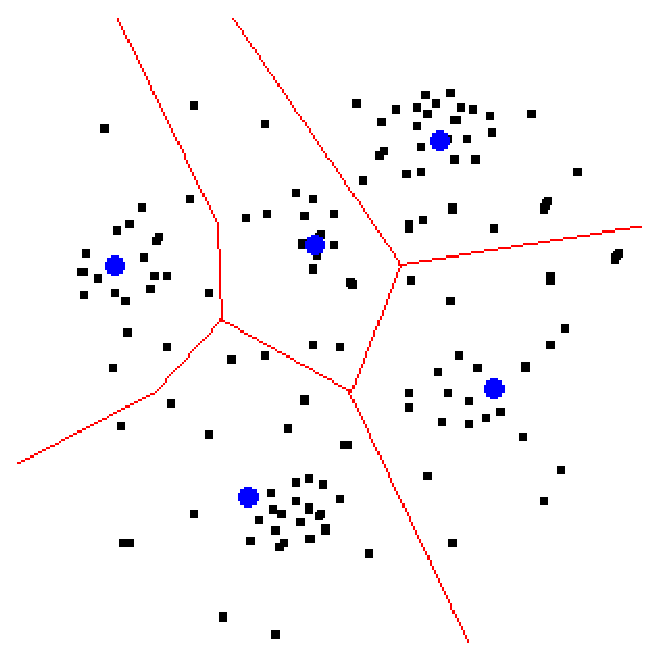
\includegraphics[width=0.4\textwidth]{kmeans1}
    \caption{kmeans}\label{fig:kmeans1}
    \vspace{\baselineskip}
    \end{figure}

\section{算法}

    算法伪代码  

    step1:初始化聚类分组的数目

    step2:初始化分组,确定每个分组的中心点

    step3:对于每个数据点进行以下操作

            step4: 确定当前数据点到每个分组中心点的距离

            step5:对比当前数据点到每个分组中心的距离,将当前数据点归类于距离某个分组中心点距离最小的分组中去

            step6: 更新每个分组的中心,如有变化,跳至step3,当中心点不再发生变化时,跳至step7

    step7:结束整个算法      
            
\section{算法伪代码}

   kmeans算法流程图如图~\ref{fig:kmeans2}所示

    \begin{figure}[htbp]
    \centering
    \includegraphics[width=0.4\textwidth]{kmeansflowchart}
    \caption{kmeans流程图}\label{fig:kmeans2}
    \vspace{\baselineskip}
    \end{figure}

\begin{algorithmic}


    \While{$\ell/N >threshold $}
    \State $\ell \gets 0$
    \For {$i \gets 0 to N-1 $}
        \For {$j \gets to   K-1 $}
        \State  $   distance \gets |objects[i]-clusters[j]|$ 
        \If{$ distance < d_{min}$} 
        \State  $ d_{min} \gets distance $
                \State $n \gets j$
            \EndIf    
        \EndFor
        \If {$membership[i] \not= n $}
            \State $\ell \gets \ell + 1$
            \State $ membership[i] \gets n$
        \EndIf
       \State $newclusters[n] \gets newclusters[n]+objects[i] $
       \State $newclustersize[n] \gets  newclustersize[n]+$1
    \EndFor
    \For{$j \gets 0 to K-1$}
       \State $clusters[j][*] \gets newclusters[j][*]/newclustersize[i] $
       \State $newclusters[j][*] \gets 0 $
       \State $newclustersize[j] \gets 0$
    \EndFor 
    \EndWhile
\end{algorithmic}
